\chapter{ANALISIS DAN PERANCANGAN SISTEM}
Bab ini akan menjelaskan analisis dan perancangan sistem untuk mencapai tujuan dari tugas akhir, meliputi perancangan data, proses, dan analisa implementasi secara umum.

\section{Analisis Sistem}
Subbab ini akan membahas mengenai hasil analisa perangkat lunak \textit{push notification} terpusat.
Analisis yang dilakukan meliputi analisis permasalahan, deskripsi umum sistem, dan spesifikasi kebutuhan perangkat lunak.

\subsection{Analisis Permasalahan}
Permasalahan yang diangkat pada tugas akhir ini adalah karena aplikasi \textit{push notification} terpusat yang digunakan saat ini kurang dapat diandalkan untuk mengirim notifikasi dalam jumlah besar.
Berdasarkan hasil pengujian yang telah dilakukan, tingkat keberhasilan pengiriman notifikasi ke 3000 pengguna hanya 63,8 persen~\cite{application-thesis}.
Rendahnya tingkat keberhasilan pengiriman ini disebabkan oleh kasus \textit{Race Condition} dalam implementasi \textit{queue} yang dibuat.

\subsection{Deskripsi Umum Sistem}
Aplikasi \textit{push notification} terpusat merupakan aplikasi yang digunakan untuk mengirim notifikasi ke perangkat pengguna secara terjadwal dan \textit{asynchronous}.
Aplikasi \textit{push notification} terpusat terbagi menjadi 3 modul, yaitu \textit{Scheduler}, \textit{Sender APN}, dan \textit{Sender FCM}.
Secara umum, \textit{Scheduler} bertanggung jawab untuk mengantrikan notifikasi yang sudah saatnya dikirim, \textit{Sender APN} bertanggung jawab untuk mengirimkan notifikasi yang diantrikan ke perangkat \textit{iOS}, dan \textit{Sender FCM} bertanggung jawab untuk mengirimkan notifikasi yang diantrikan ke perangkat \textit{Android} dan \textit{Web}.
Komunikasi antar modul aplikasi push notification terpusat menggunakan pola \textit{publish/subscribe}, dengan pembagian antrian (\textit{message queue}) berdasarkan topik.
Topik antrian dibagi berdasarkan tipe perangkat penerima notifikasi, yaitu \textit{Android}, \textit{Web}, dan \textit{iOS}.
Scheduler akan mem-\textit{publish} notifikasi ke topik antrian yang sesuai, \textit{Sender APN} akan men-\textit{subscribe} notifikasi yang ada di antrian topik \textit{iOS}, dan \textit{Sender FCM} akan men-\textit{subscribe} notifikasi yang ada di antrian topik \textit{Android} dan \textit{Web}.
Pada tugas akhir ini, Komunikasi antar modul serta penyimpanan antrian akan diatur oleh \textit{Kafka}, dan implementasi modul aplikasi push notification terpusat akan menggunakan kerangka kerja \textit{Spring} dengan bahasa pemrograman \textit{Java}.

\subsection{Spesifikasi Kebutuhan Perangkat Lunak}
Subbab ini membahas spesifikasi kebutuhan perangkat lunak dari hasil analisis yang telah dilakukan.
Subbab ini berisi kebutuhan perangkat lunak yang direpresentasikan dalam bentuk kebutuhan fungsional, kebutuhan non fungsional, dan diagram kasus penggunaan.

\subsubsection{Aktor}
\begin{longtable}{|p{2cm}|p{6cm}|}
    \hline
    \textbf{Aktor} & \textbf{Tugas} & \hline
    \textit{Scheduler} & Membuat dan menjadwalkan pengiriman packet notifikasi. & \hline
    \textit{Sender APN} & Mengirimkan packet notifikasi untuk perangkat \textit{iOS}. & \hline
    \textit{Sender FCM} & Mengirimkan packet notifikasi untuk perangkat \textit{Android} dan \textit{Web}. & \hline
    \caption{Aktor pada sistem}
\end{longtable}

\subsubsection{Kebutuhan Fungsional}
\begin{longtable}{|p{2.5cm}|p{2cm}|p{4.5cm}|}
    \hline
    \textbf{No.} & \textbf{Kebutuhan Fungsional} & \textbf{Deskripsi} & \hline
    F01 & Mengirim notifikasi ke beberapa akun & Sistem dapat mengirim notifikasi ke perangkat Android, Web, dan iOS yang dimiliki oleh akun tertentu. & \hline
    F02 & Mengirim notifikasi ke beberapa grup & Sistem dapat mengirim notifikasi ke perangkat Android, Web, dan iOS yang dimiliki oleh akun yang merupakan anggota dari grup tertentu. & \hline
    F03 & Mengirim notifikasi secara terjadwal & Sistem dapat mengirim notifikasi ke perangkat Android, Web, dan iOS pada waktu tertentu. & \hline
    F04 & Menyimpan hasil pengiriman notifikasi & Sistem dapat menyimpan hasil pengiriman (\textit{response} dari \textit{APNs}, \textit{FCM}, atau \textit{error stacktrace}) setiap notifikasi yang dikirim. & \hline
    \caption{Kebutuhan fungsional sistem}
\end{longtable}

\subsubsection{Kebutuhan Non Fungsional}
\begin{longtable}{|p{0.5cm}|p{2cm}|p{5.5cm}|}
    \hline
    \textbf{No.} & \textbf{Parameter} & \textbf{Deskripsi} & \hline
    1 & Reliability & Aplikasi dapat mengirimkan 100.000 notifikasi ke layanan FCM \& APNs dengan tingkat keberhasilan 90 persen. & \hline
    2 & Portability & Aplikasi dapat dijalankan pada sistem operasi berbasis linux. & \hline
    3 & Availability & Aplikasi dapat menangani pengiriman 100.000 notifikasi tanpa \textit{down}. & \hline
    \caption{Kebutuhan non fungsional sistem}
\end{longtable}

\subsubsection{Diagram Kasus Penggunaan}
\par Subbab ini menjelaskan kasus penggunaan perangkat lunak secara rinci. Kasus penggunaan dibuat berdasarkan hasil analisis yang pada subbab sebelumnya.
\par Diagram kasus penggunaan untuk setiap modul (\textit{Scheduler}, \textit{Sender APN}, dan \textit{Sender FCM}) aplikasi \textit{push notification} terpusat dapat dilihat pada diagram~\ref{diagram_kasus_penggunaan}.
\begin{figure}[H]
    \centering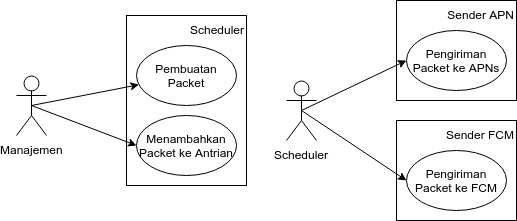
\includegraphics[width=1\textwidth]{bab3/figures/diagram_kasus_penggunaan.jpg}
    \caption{Diagram Kasus Penggunaan}
    \label{diagram_kasus_penggunaan}
\end{figure}
Penjelasan lebih lengkap dapat dilihat pada tabel~\ref{tabel_deskripsi_kasus_penggunaan_sistem}.
\begin{longtable}{|p{1cm}|p{5.5cm}|p{2cm}|}
    \hline
    \textbf{Kode} & \textbf{Nama Kasus Penggunaan} & \textbf{Aktor} & \hline
    UC01 & Pembuatan Packet & Scheduler & \hline
    UC02 & Menambahkan Packet ke Antrian & Scheduler & \hline
    UC03 & Pengiriman Packet ke APNs & Sender APN & \hline
    UC04 & Pengiriman Packet ke FCM & Sender FCM & \hline
    \caption{Deskripsi Kasus Penggunaan Sistem}
    \label{tabel_deskripsi_kasus_penggunaan_sistem}
\end{longtable}

% template tabel deskripsi kasus penggunaan
\newcommand\tableUcDesc[7] {
\begin{longtable}{|p{2.5cm}|p{6.5cm}|}
    \hline
    \textbf{Komponen} & \textbf{Deskripsi} & \hline
    Kode & #1 & \hline
    Nama & #2 & \hline
    Deskripsi & #3 & \hline
    Aktor & #4 & \hline
    Kondisi Awal & #5 & \hline
    Kondisi Akhir & #6 & \hline
    Alur Normal & #7 & \hline
    \caption{Kasus Penggunaan #2}
\end{longtable}
}

\paragraph{Pembuatan Packet}
\par Pada kasus ini, \textit{Scheduler} akan memeriksa secara berkala apakah terdapat batch yang belum di proses.
Jika ada, \textit{Scheduler} akan membuatkan \textit{packet} untuk \textit{batch} tersebut.
\tableUcDesc
{UC01}
{Pembuatan Packet}
{Packet akan dibuat setiap ada batch baru di database}
{Scheduler}
{Batch ditambahkan ke database}
{Packet ditambahkan ke database}
{
\begin{enumerate}
    \item Aktor memeriksa apakah terdapat batch yang belum di proses di database.
    \item Aktor membuat data packet dari data batch tersebut.
    \item Aktor menyimpan data packet dan memperbarui data batch di database.
\end{enumerate}
}

\paragraph{Menambahkan Packet ke Antrian}
\par Pada kasus ini, Scheduler akan memeriksa pada interval waktu tertentu apakah ada packet yang sudah waktunya untuk
dikirim.
Jika ada, scheduler akan menambahkan packet tersebut ke antrian kafka dengan topik yang sesuai.
\tableUcDesc
{UC02}
{Menambahkan Packet ke Antrian}
{Packet akan diantrikan ke kafka sesuai dengan jadwal pengiriman dan topik (Android, Web, atau iOS)}
{Scheduler}
{1 menit setelah pengecekan terakhir}
{Packet diantrikan ke kafka}
{
\begin{enumerate}
    \item Aktor memeriksa apakah terdapat packet yang sudah waktunya dikirim di database.
    \item Aktor menambahkan packet ke dalam antrian kafka dengan spesifikasi topik sebagai berikut:
    \begin{enumerate}
        \item Topik "android" untuk packet dengan target perangkat Android.
        \item Topik "web" untuk packet dengan target perangkat Web.
        \item Topik "ios" untuk packet dengan target perangkat iOS.
    \end{enumerate}
    \item Aktor memperbarui data packet di database.
\end{enumerate}
}

\paragraph{Pengiriman Packet ke APNs}
\par Pada kasus ini, Sender APN akan menunggu Kafka untuk mengirimkan packet yang berada dalam antrian topik "ios".
Setelah packet diterima, packet akan dikirim ke layanan APNs, dan kemudian akan diterima oleh perangkat pengguna.
\tableUcDesc
{UC03}
{Pengiriman Packet ke APNs}
{Packet yang ada didalam antrian topik "ios" akan dikirimkan ke layanan APNs}
{Sender APN}
{Packet diterima dari antrian topik "ios" di Kafka}
{Packet diterima oleh APNs}
{
\begin{enumerate}
    \item Aktor menunggu packet dari antrian topik "ios" di kafka.
    \item Aktor mengirimkan request notifikasi ke layanan APNs berdasarkan data packet.
    \item Aktor memperbarui data packet di database berdasarkan response dari APNs.
\end{enumerate}
}

\paragraph{Pengiriman Packet ke FCM}
\par Pada kasus ini, Sender FCM akan menunggu Kafka untuk mengirimkan packet yang berada dalam antrian topik "android" dan "web".
Setelah packet diterima, packet akan dikirim ke layanan FCM, dan kemudian akan diterima oleh perangkat pengguna.
\tableUcDesc
{UC04}
{Pengiriman Packet ke FCM}
{Packet yang ada didalam antrian topik "android" akan dikirimkan ke layanan FCM}
{Sender FCM}
{Packet diterima dari antrian topik "android" atau "web" di kafka}
{Packet diterima oleh FCM}
{
\begin{enumerate}
    \item Aktor menunggu packet dari antrian topik "android" atau "web" di kafka.
    \item Aktor mengirimkan request notifikasi ke layanan FCM berdasarkan data packet.
    \item Aktor memperbarui data packet di database berdasarkan response dari FCM.
\end{enumerate}
}

\section{Perancangan Sistem}
\par Subbab ini akan membahas tahapan perancangan sistem yang dibagi menjadi beberapa bagian, yaitu perancangan
arsitektur, data, dan proses.

\subsection{Perancangan Arsitektur}
\par Aplikasi \textit{push notification} terpusat akan dibagi menjadi 3 modul, yaitu \textit{Scheduler},
\textit{Sender APN}, dan \textit{Sender FCM}.
Aplikasi dibangun dengan bahasa pemrograman Java, dengan kerangka kerja
Spring.
Aplikasi saling terhubung lewat Kafka dan SQL Server.
Secara garis besar, aplikasi ini memiliki rancangan
arsitektur pengiriman notifikasi yang dapat dilihat pada gambar~\ref{arsitektur_pengiriman_notifikasi}.
\begin{figure}[H]
    \centering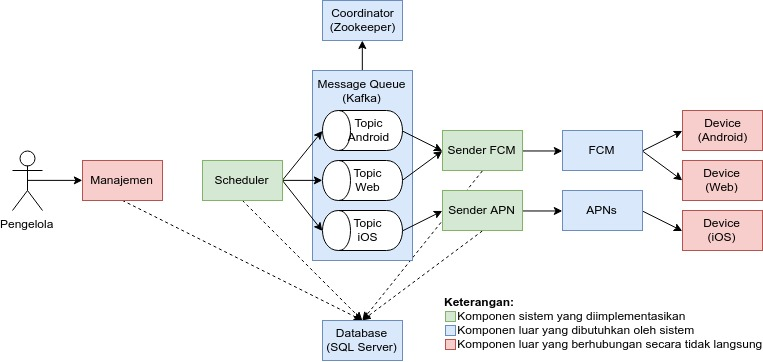
\includegraphics[width=1\textwidth]{bab3/figures/arsitektur_pengiriman_notifikasi.jpg}
    \caption{Arsitektur Pengiriman Notifikasi}
    \label{arsitektur_pengiriman_notifikasi}
\end{figure}

\subsection{Perancangan Basis Data}
\par Subbab ini membahas bagaimana rancangan basis data yang digunakan pada aplikasi \textit{push notification}
terpusat.
Basis data yang digunakan adalah SQL Server 2012.

\subsubsection{Tabel User (user\_account)}
\par Tabel ini digunakan untuk menyimpan data pengguna aplikasi yang ada di Institut Teknologi Sepuluh Nopember. Detail atribut dapat dilihat pada tabel berikut.
\begin{longtable}{|p{2.5cm}|p{2cm}|p{4.5cm}|}
    \hline
    \textbf{Nama Atribut} & \textbf{Tipe Data} & \textbf{Deskripsi} & \hline
    User ID & uuid & Primary key tabel & \hline
    Created At & datetime & Tanggal dan waktu dibuat & \hline
    Update At & datetime & Tanggal dan waktu diperbarui & \hline
    \caption{Tabel User (user\_account)}
\end{longtable}

\subsubsection{Tabel Group (pn\_group)}
\par Tabel ini digunakan untuk mengelompokan pengguna. Detail atribut dapat dilihat pada tabel berikut.
\begin{longtable}{|p{2.5cm}|p{2cm}|p{4.5cm}|}
    \hline
    \textbf{Nama Atribut} & \textbf{Tipe Data} & \textbf{Deskripsi} & \hline
    Group ID & uuid & Primary key tabel & \hline
    Created At & datetime & Tanggal dan waktu dibuat & \hline
    Update At & datetime & Tanggal dan waktu diperbarui & \hline
    \caption{Tabel Group (pn\_group)}
\end{longtable}

\subsubsection{Tabel Group Member (pn\_group\_member)}
\par Tabel ini digunakan untuk menambahkan pengguna kedalam suatu kelompok. Detail atribut dapat dilihat pada tabel berikut.
\begin{longtable}{|p{2.5cm}|p{2cm}|p{4.5cm}|}
    \hline
    \textbf{Nama Atribut} & \textbf{Tipe Data} & \textbf{Deskripsi} & \hline
    Group ID & uuid & Grup tempat pengguna terdaftar & \hline
    User ID & uuid & Pengguna yang terdaftar di grup & \hline
    Created At & datetime & Tanggal dan waktu dibuat & \hline
    Update At & datetime & Tanggal dan waktu diperbarui & \hline
    \caption{Tabel Group Member (pn\_group\_member)}
\end{longtable}

\subsubsection{Tabel Client (oauth\_client)}
\par Tabel ini digunakan untuk menyimpan data \textit{client} (aplikasi) yang ada di Institut Teknologi Sepuluh Nopember. Detail atribut dapat dilihat pada tabel berikut.
\begin{longtable}{|p{2.5cm}|p{2cm}|p{4.5cm}|}
    \hline
    \textbf{Nama Atribut} & \textbf{Tipe Data} & \textbf{Deskripsi} & \hline
    Client ID & uuid & Primary key tabel & \hline
    Created At & datetime & Tanggal dan waktu dibuat & \hline
    Update At & datetime & Tanggal dan waktu diperbarui & \hline
    \caption{Tabel Client (oauth\_client)}
\end{longtable}

\subsubsection{Tabel Certificate (pn\_certificate)}
\par Tabel ini digunakan untuk menyimpan data sertifikat yang digunakan untuk autentikasi ke layanan APNs dan FCM. Detail atribut dapat dilihat pada tabel berikut.
\begin{longtable}{|p{2.5cm}|p{2cm}|p{4.5cm}|}
    \hline
    \textbf{Nama Atribut} & \textbf{Tipe Data} & \textbf{Deskripsi} & \hline
    Certificate ID & uuid & Primary key tabel & \hline
    Client ID & uuid & Foreign key tabel client & \hline
    Bundle ID & varchar(255) & Bundle ID untuk aplikasi iOS & \hline
    Certificate Key & text & File sertifikat yang sudah diencode dengan base64 & \hline
    Type & char(1) & Tipe sertifikat (FCM atau APNs) & \hline
    Password & varchar(255) & Kata sandi untuk sertifikat iOS & \hline
    Created At & datetime & Tanggal dan waktu dibuat & \hline
    Update At & datetime & Tanggal dan waktu diperbarui & \hline
    \caption{Tabel Certificate (pn\_certificate)}
\end{longtable}

\subsubsection{Tabel Device (device\_token)}
\par Tabel ini digunakan untuk menyimpan data perangkat pengguna yang terdaftar di layanan APNs dan FCM. Detail atribut dapat dilihat pada tabel berikut.
\begin{longtable}{|p{2.5cm}|p{2cm}|p{4.5cm}|}
    \hline
    \textbf{Nama Atribut} & \textbf{Tipe Data} & \textbf{Deskripsi} & \hline
    Device ID & uuid & Primary key tabel & \hline
    Client ID & uuid & Client tempat perangkat terdaftar & \hline
    User ID & uuid & User pemilik perangkat & \hline
    Device Token & varchar(255) & Token yang terdaftar di layanan APNs dan FCM & \hline
    Device Type & char(1) & Jenis perangkat (Android, Web, atau iOS) & \hline
    Active & numeric(1) & Perangkat aktif atau tidak & \hline
    Created At & datetime & Tanggal dan waktu dibuat & \hline
    Update At & datetime & Tanggal dan waktu diperbarui & \hline
    \caption{Tabel Device (device\_token)}
\end{longtable}

\subsubsection{Tabel Batch (pn\_batch)}
\par Tabel ini digunakan untuk menyimpan data notifikasi yang akan dikirim ke beberapa perangkat. Detail atribut dapat dilihat pada tabel berikut.
\begin{longtable}{|p{2.5cm}|p{2cm}|p{4.5cm}|}
    \hline
    \textbf{Nama Atribut} & \textbf{Tipe Data} & \textbf{Deskripsi} & \hline
    Batch ID & uuid & Primary key tabel & \hline
    Title & varchar(255) & Judul notifikasi & \hline
    Body & varchar(255) & Isi pesan notifikasi & \hline
    Image & varchar(255) & Nama atau URL Gambar & \hline
    Sound & varchar(255) & Nama atau URL Suara & \hline
    Action & varchar(255) & Nama aksi yang dijalankan jika notifikasi dibuka & \hline
    Additional Data & varchar(255) & Data tambahan dengan format JSON & \hline
    Delivery Date & datetime & Waktu notifikasi dikirim & \hline
    Started Date & datetime & Waktu batch mulai diproses & \hline
    Finished Date & datetime & Waktu batch selesai diproses & \hline
    Is Allowed & numeric(1) & Batch boleh diproses atau tidak & \hline
    User Sender ID & uuid & User pembuat batch & \hline
    Client Sender ID & uuid & Client pembuat batch & \hline
    Client Destination ID & uuid & Client tujuan penerima notifikasi & \hline
    Created At & datetime & Tanggal dan waktu dibuat & \hline
    Update At & datetime & Tanggal dan waktu diperbarui & \hline
    \caption{Tabel Batch (pn\_batch)}
\end{longtable}

\subsubsection{Tabel Packet (pn\_packet)}
\par Tabel ini digunakan untuk menyimpan data notifikasi yang dikirim ke satu perangkat. Detail atribut dapat dilihat pada tabel berikut.
\begin{longtable}{|p{2.5cm}|p{2cm}|p{4.5cm}|}
    \hline
    \textbf{Nama Atribut} & \textbf{Tipe Data} & \textbf{Deskripsi} & \hline
    Packet ID & uuid & Primary key tabel & \hline
    Batch ID & uuid & Batch notifikasi & \hline
    Device Token ID & uuid & Perangkat penerima notifikasi & \hline
    Sent At & datetime & Waktu notifikasi diterima oleh APNs atau FCM & \hline
    Reason & varchar(255) & Penyebab jika terjadi kegagalan & \hline
    Packet Status & numeric(1) & Status pengiriman packet (dibuat, menunggu, berhasil, atau gagal) & \hline
    Created At & datetime & Tanggal dan waktu dibuat & \hline
    Update At & datetime & Tanggal dan waktu diperbarui & \hline
    \caption{Tabel Packet (pn\_packet)}
\end{longtable}

\subsubsection{Tabel User Destination (pn\_user\_destination)}
\par Tabel ini digunakan untuk menyimpan data pengguna yang menjadi target penerima notifikasi dalam satu \textit{batch}. Detail atribut dapat dilihat pada tabel berikut.
\begin{longtable}{|p{2.5cm}|p{2cm}|p{4.5cm}|}
    \hline
    \textbf{Nama Atribut} & \textbf{Tipe Data} & \textbf{Deskripsi} & \hline
    Batch ID & uuid & Batch notifikasi & \hline
    User ID & uuid & Pengguna penerima notifikasi & \hline
    Created At & datetime & Tanggal dan waktu dibuat & \hline
    Update At & datetime & Tanggal dan waktu diperbarui & \hline
    \caption{Tabel User Destination (pn\_user\_destination)}
\end{longtable}

\subsubsection{Tabel Group Destination (pn\_group\_destination)}
\par Tabel ini digunakan untuk menyimpan data kelompok yang menjadi target penerima notifikasi dalam satu \textit{batch}. Detail atribut dapat dilihat pada tabel berikut.
\begin{longtable}{|p{2.5cm}|p{2cm}|p{4.5cm}|}
    \hline
    \textbf{Nama Atribut} & \textbf{Tipe Data} & \textbf{Deskripsi} & \hline
    Batch ID & uuid & Batch notifikasi & \hline
    Group ID & uuid & Grup penerima notifikasi & \hline
    Created At & datetime & Tanggal dan waktu dibuat & \hline
    Update At & datetime & Tanggal dan waktu diperbarui & \hline
    \caption{Tabel Group Destination (pn\_group\_destination)}
\end{longtable}

\subsection{Perancangan Proses}
\par Subbab ini menjelaskan tentang rancangan, tujuan, dan diagram alir proses-proses yang ada pada aplikasi
\textit{push notification} terpusat.

\subsubsection{Proses Pembuatan Packet}
\par Proses ini bertujuan untuk membuat \textit{packet} dari \textit{batch} yang baru dibuat.
Proses pembuatan dapat
dilihat di diagram alir pada gambar~\ref{flowchart_pembuatan_packet}.
\begin{figure}[H]
    \centering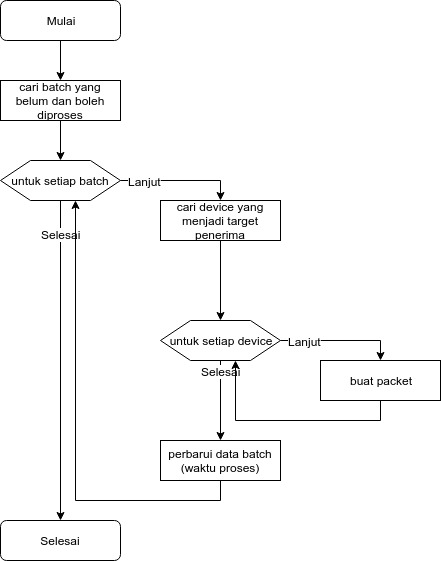
\includegraphics[width=0.8\textwidth]{bab3/figures/flowchart_pembuatan_packet.jpg}
    \caption{Diagram Alir Proses Pembuatan \textit{Packet}}
    \label{flowchart_pembuatan_packet}
\end{figure}

\subsubsection{Proses Menambahkan Packet ke Antrian}
\par Proses ini bertujuan untuk mengantrikan \textit{packet} yang sudah waktunya untuk dikirim.
Antrian
\textit{packet} dibagi berdasarkan jenis perangkat penerima notifikasi (Android, Web, atau iOS).
Proses pengantrian
dapat dilihat di diagram alir pada gambar~\ref{flowchart_menambahkan_packet_ke_antrian}.
\begin{figure}[H]
    \centering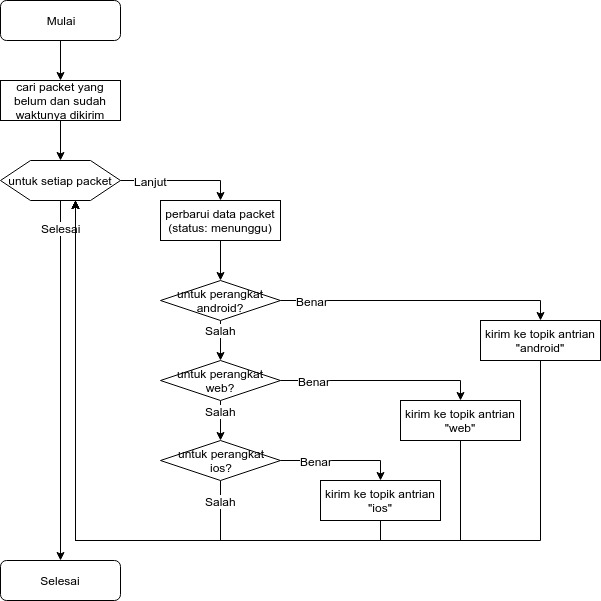
\includegraphics[width=0.7\textwidth]{bab3/figures/flowchart_menambahkan_packet_ke_antrian.jpg}
    \caption{Diagram Alir Proses Menambahkan \textit{Packet} ke Antrian}
    \label{flowchart_menambahkan_packet_ke_antrian}
\end{figure}

\subsubsection{Proses Pengiriman Packet ke APNs}
\par Proses ini bertujuan untuk mengirimkan \textit{packet} yang ada di antrian topik "ios" ke perangkat pengguna
yang berbasis iOS lewat layanan APNs. Proses pengiriman \textit{packet} dapat dilihat di diagram alir pada
gambar~\ref{flowchart_pengiriman_packet_ke_apns}.
\begin{figure}[H]
    \centering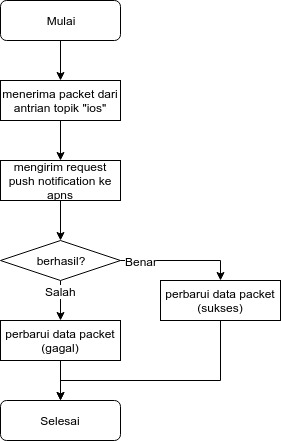
\includegraphics[width=0.7\textwidth]{bab3/figures/flowchart_pengiriman_packet_ke_apns.jpg}
    \caption{Diagram Alir Proses Pengiriman \textit{Packet} ke APNs}
    \label{flowchart_pengiriman_packet_ke_apns}
\end{figure}
\linebreak

\subsubsection{Proses Pengiriman Packet ke FCM}
\par Proses ini bertujuan untuk mengirimkan \textit{packet} yang ada di antrian topik "android" dan "web" ke
perangkat pengguna yang berbasis Android atau Web lewat layanan FCM. Proses pengiriman \textit{packet} dapat dilihat di
diagram alir pada gambar~\ref{flowchart_pengiriman_packet_ke_fcm}.
\begin{figure}[H]
    \centering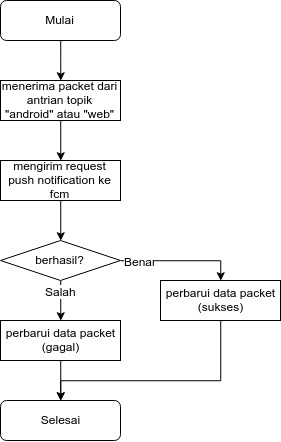
\includegraphics[width=0.7\textwidth]{bab3/figures/flowchart_pengiriman_packet_ke_fcm.jpg}
    \caption{Diagram Alir Proses Pengiriman \textit{Packet} ke FCM}
    \label{flowchart_pengiriman_packet_ke_fcm}
\end{figure}
\linebreak
